\documentclass[10pt,a4paper]{article}
\usepackage[utf8]{inputenc}
\usepackage[german]{babel}
\usepackage{amsmath}
\usepackage{amsfonts}
\usepackage{amssymb}
\usepackage{siunitx}
\usepackage{multirow}
\usepackage[left=2cm,right=2cm,top=2cm,bottom=2cm]{geometry}
\usepackage{wrapfig}
\usepackage{graphicx}
\usepackage[outdir=./]{epstopdf}
\usepackage{caption}
\usepackage[colorlinks]{hyperref}


\author{Christian Bespin \and Christopher Deutsch}
\title{Übungsblatt 3: Numerische Methoden der Physik}
\begin{document}
\maketitle

\setcounter{section}{1}

\section{Treibhauseffekt}

\subsection{Physikalischer Hintergrund}
Zur Erklärung des Treibhauseffektes wird ein Modell grauer und schwarzer Körper
im thermischen Gleichgewicht verwendet. Wir beschreiben die Erde als schwarzen
Strahler mit Emissions-/Absorptionsgrad $\epsilon_E = \alpha_E = 1$. Die Sonne 
wird durch einen grauen Strahler der Temperatur $T_S$ mit Emissionsgrad
$\epsilon_S = \text{konst.}$ ersetzt.
Auch die Atmosphäre wird als grauer Strahler modelliert. Diese habe die
Temperatur $\tau$ und den Emissionsgrad $\epsilon(\tau)$. 
Das Kirchhoff'sche Strahlungsgesetz besagt, dass der Emissionsgrad $\epsilon$ eines
grauen Körpers gleich seinem Absorptionsgrad $\alpha$ ist. Demnach hat die
Atmosphäre für Strahlung der Temperatur $T$ den Absorptionsgrad $\alpha(\tau) = \epsilon(\tau)$.

\begin{wrapfigure}[14]{R}[1pt]{0.47\textwidth}
\centering
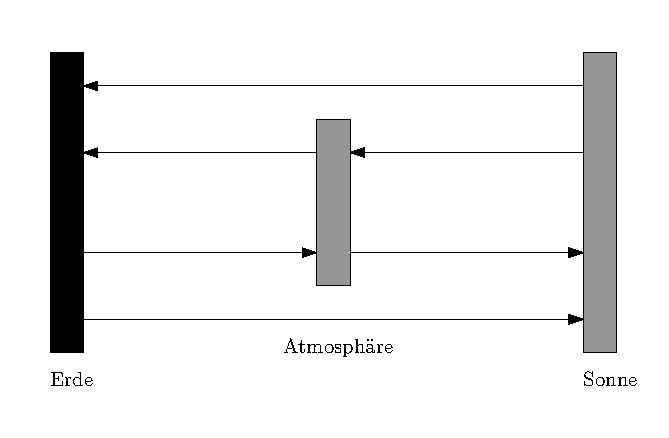
\includegraphics[width=0.45\textwidth]{./figures/strahlungsgleichgewicht.eps}
\caption{Strahlungsgleichgewicht}
\label{fig:strahlungsgleichgewicht}
\end{wrapfigure}
\noindent Ein Körper ist im thermischen Gleichgewicht, wenn seine abgestrahlte Leistung
gleich seiner absorbierten Leistung ist. Diese wird durch das Stefan-Boltzmann-Gesetz
$P \propto \epsilon T^4$ beschrieben. Die Gleichgewichtsbedingung für die Atmosphäre ist:
\begin{align}
	2\epsilon(\tau)\tau^4 &= \alpha(T_S) \epsilon_S T_S^4 + \alpha(T_E) \epsilon_E T_E^4 \notag \\ &=\epsilon(T_S) \epsilon_S T_S^4 + \epsilon(T_E) T_E^4
\end{align}
Dabei wurde die Proportionalitätskonstante aus der Gleichung heraus gekürzt.
Der Term auf der linken Seite beschreibt die Abstrahlung der Atmosphäre, wobei
Faktor $2$ die Abstrahlung sowohl zur Erde als auch zur Sonne beschreibt.
Die rechte Seite beschreibt die Absorption, dabei wurde erst im letzten
Umformungsschritt $\epsilon_E = 1$ und das Kirchhoff'sche Strahlungsgesetz verwendet,
um den Unterschied zwischen der Absorption der Atmosphäre und des Emissionsgrades von
Sonne/Erde deutlich zu machen.
Analog dazu erhält man zwei weitere Gleichgewichtsbedingungen, aus denen man
$\tau$ eliminieren kann und eine Bestimmungsgleichung für die Temperatur $T_E$
der Erde im Gleichgewicht erhält:
\begin{align}
\left[2-\epsilon(T_E)\right]T_E^4=\epsilon_S\left[2-\epsilon(T_S)\right]T_S^4
\end{align}

$\nu_{max}=T\cdot 5,8789254\num{1E10}\si{\per\second}\si{\per\kelvin}$ \footnote{http://physics.nist.gov/constants, Wien frequency displacement law constant}

\subsection{Mathematischer Hintergrund}

\subsection{Implementierung}

Das Programm besteht aus zwei Teilen: der numerischen Integration, bei der $epsilon(T)$ bestimmt wird und der numerischen Auswertung, um $T_E$ zu bestimmen, bei der INSERT GLEICHUNGSNUMMERgilt.

Z wurde analytisch berechnet: $Z=\frac{8}{15}\frac{\pi^5 \mathrm{kT}}{\mathrm{c}^3}$

\subsubsection{Nullstellenberechnung mit Bisektion}

Ein Verfahren, um numerisch Nullstellen zu bestimmen, ist das 1-Punkt-Iterationsverfahren Bisektion. Wir verwenden dieses hier, da es im Gegensatz zum Newtonverfahren keine Ableitungen der Funktion berechnen und auswerten muss. Dabei wird vorausgesetzt, dass die Funktion auf dem relevanten Intervall $[a,b]$ nur eine Nullstelle hat. Die Bisektion halbiert das zu betrachtende Intervall immer so, dass der Vorzeichenwechsel des Funktionswerts im betrachteten Intervall bleibt. Der Fehler halbiert sich mit jedem Iterationsschritt, was nicht so schnell wie das Newtonverfahren ist, die Laufzeit des Programms aber dennoch in einem akzeptablen Rahmen hält.
\begin{figure}[tbp]
\centering
\includegraphics[width=0.6\textwidth]{./figures/bisektion.eps}
\caption{Bisektions-Verfahren}
\label{fig:bisektion}
\end{figure}

\subsubsection{Numerische Integration mit rekursivem Simpson-Verfahren}

Wir verwenden zur numerischen Integration eine rekursive Variante des Simpson-Verfahrens, bei der das Intervall, über dem integriert wird, mit jedem Rekursionsschritt in zwei Hälften zerlegt wird, auf die die normale Simpson-Methode angewendet wird. Ist die Differenz zwischen dem mit Simpson über dem ganzen Intervall berechneten Integralwert und der Summe der zwei Teilintervalle größer als eine vorgegebene Genauigkeit, wird die Funktion rekursiv aufgerufen, wodurch jedes der Teilintervalle erneut halbiert wird. Durch dieses Vorgehen fallen im Gegensatz zum gewöhnlichen Simpsonverfahren einige laufzeitbeeinträchtigende Funktionsaufrufe weg.

\subsubsection{Abbruchbedingungen}

Integrationsgrenzen
\begin{figure}[htbp]
\centering
\input{./figures/rho}
\caption{Integrand für T=300K}
\end{figure}

\begin{figure}[htbp]
\centering
% GNUPLOT: LaTeX picture with Postscript
\begingroup
  \makeatletter
  \providecommand\color[2][]{%
    \GenericError{(gnuplot) \space\space\space\@spaces}{%
      Package color not loaded in conjunction with
      terminal option `colourtext'%
    }{See the gnuplot documentation for explanation.%
    }{Either use 'blacktext' in gnuplot or load the package
      color.sty in LaTeX.}%
    \renewcommand\color[2][]{}%
  }%
  \providecommand\includegraphics[2][]{%
    \GenericError{(gnuplot) \space\space\space\@spaces}{%
      Package graphicx or graphics not loaded%
    }{See the gnuplot documentation for explanation.%
    }{The gnuplot epslatex terminal needs graphicx.sty or graphics.sty.}%
    \renewcommand\includegraphics[2][]{}%
  }%
  \providecommand\rotatebox[2]{#2}%
  \@ifundefined{ifGPcolor}{%
    \newif\ifGPcolor
    \GPcolortrue
  }{}%
  \@ifundefined{ifGPblacktext}{%
    \newif\ifGPblacktext
    \GPblacktextfalse
  }{}%
  % define a \g@addto@macro without @ in the name:
  \let\gplgaddtomacro\g@addto@macro
  % define empty templates for all commands taking text:
  \gdef\gplbacktext{}%
  \gdef\gplfronttext{}%
  \makeatother
  \ifGPblacktext
    % no textcolor at all
    \def\colorrgb#1{}%
    \def\colorgray#1{}%
  \else
    % gray or color?
    \ifGPcolor
      \def\colorrgb#1{\color[rgb]{#1}}%
      \def\colorgray#1{\color[gray]{#1}}%
      \expandafter\def\csname LTw\endcsname{\color{white}}%
      \expandafter\def\csname LTb\endcsname{\color{black}}%
      \expandafter\def\csname LTa\endcsname{\color{black}}%
      \expandafter\def\csname LT0\endcsname{\color[rgb]{1,0,0}}%
      \expandafter\def\csname LT1\endcsname{\color[rgb]{0,1,0}}%
      \expandafter\def\csname LT2\endcsname{\color[rgb]{0,0,1}}%
      \expandafter\def\csname LT3\endcsname{\color[rgb]{1,0,1}}%
      \expandafter\def\csname LT4\endcsname{\color[rgb]{0,1,1}}%
      \expandafter\def\csname LT5\endcsname{\color[rgb]{1,1,0}}%
      \expandafter\def\csname LT6\endcsname{\color[rgb]{0,0,0}}%
      \expandafter\def\csname LT7\endcsname{\color[rgb]{1,0.3,0}}%
      \expandafter\def\csname LT8\endcsname{\color[rgb]{0.5,0.5,0.5}}%
    \else
      % gray
      \def\colorrgb#1{\color{black}}%
      \def\colorgray#1{\color[gray]{#1}}%
      \expandafter\def\csname LTw\endcsname{\color{white}}%
      \expandafter\def\csname LTb\endcsname{\color{black}}%
      \expandafter\def\csname LTa\endcsname{\color{black}}%
      \expandafter\def\csname LT0\endcsname{\color{black}}%
      \expandafter\def\csname LT1\endcsname{\color{black}}%
      \expandafter\def\csname LT2\endcsname{\color{black}}%
      \expandafter\def\csname LT3\endcsname{\color{black}}%
      \expandafter\def\csname LT4\endcsname{\color{black}}%
      \expandafter\def\csname LT5\endcsname{\color{black}}%
      \expandafter\def\csname LT6\endcsname{\color{black}}%
      \expandafter\def\csname LT7\endcsname{\color{black}}%
      \expandafter\def\csname LT8\endcsname{\color{black}}%
    \fi
  \fi
  \setlength{\unitlength}{0.0500bp}%
  \begin{picture}(7200.00,4320.00)%
    \gplgaddtomacro\gplbacktext{%
      \csname LTb\endcsname%
      \put(1210,704){\makebox(0,0)[r]{\strut{} 0}}%
      \put(1210,1076){\makebox(0,0)[r]{\strut{} 1}}%
      \put(1210,1449){\makebox(0,0)[r]{\strut{} 2}}%
      \put(1210,1821){\makebox(0,0)[r]{\strut{} 3}}%
      \put(1210,2193){\makebox(0,0)[r]{\strut{} 4}}%
      \put(1210,2566){\makebox(0,0)[r]{\strut{} 5}}%
      \put(1210,2938){\makebox(0,0)[r]{\strut{} 6}}%
      \put(1210,3310){\makebox(0,0)[r]{\strut{} 7}}%
      \put(1210,3683){\makebox(0,0)[r]{\strut{} 8}}%
      \put(1210,4055){\makebox(0,0)[r]{\strut{} 9}}%
      \put(1342,484){\makebox(0,0){\strut{} 1e+13}}%
      \put(4073,484){\makebox(0,0){\strut{} 1e+14}}%
      \put(6803,484){\makebox(0,0){\strut{} 1e+15}}%
      \put(176,2379){\rotatebox{-270}{\makebox(0,0){\strut{}$\rho(\nu,T=5750\,\si{\kelvin})(1-f(\nu))$ [$10^{-16}$\,\si{\joule\per\cubic\meter}]}}}%
      \put(4072,154){\makebox(0,0){\strut{}$\nu$ [\si{\per\second}]}}%
      \put(4072,3945){\makebox(0,0){\strut{}}}%
    }%
    \gplgaddtomacro\gplfronttext{%
      \csname LTb\endcsname%
      \put(2398,3882){\makebox(0,0)[r]{\strut{}$\tilde{n}=0.1$}}%
      \csname LTb\endcsname%
      \put(2398,3662){\makebox(0,0)[r]{\strut{}$\tilde{n}=1$}}%
      \csname LTb\endcsname%
      \put(2398,3442){\makebox(0,0)[r]{\strut{}$\tilde{n}=10$}}%
      \csname LTb\endcsname%
      \put(2398,3222){\makebox(0,0)[r]{\strut{}$\tilde{n}=100$}}%
    }%
    \gplbacktext
    \put(0,0){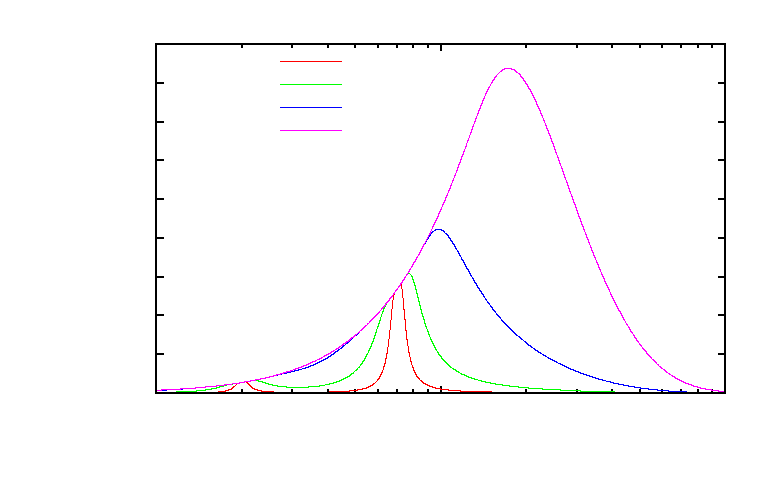
\includegraphics{./figures/rho_sonne}}%
    \gplfronttext
  \end{picture}%
\endgroup

\caption{Integrand für T=5750K}

% GNUPLOT: LaTeX picture with Postscript
\begingroup
  \makeatletter
  \providecommand\color[2][]{%
    \GenericError{(gnuplot) \space\space\space\@spaces}{%
      Package color not loaded in conjunction with
      terminal option `colourtext'%
    }{See the gnuplot documentation for explanation.%
    }{Either use 'blacktext' in gnuplot or load the package
      color.sty in LaTeX.}%
    \renewcommand\color[2][]{}%
  }%
  \providecommand\includegraphics[2][]{%
    \GenericError{(gnuplot) \space\space\space\@spaces}{%
      Package graphicx or graphics not loaded%
    }{See the gnuplot documentation for explanation.%
    }{The gnuplot epslatex terminal needs graphicx.sty or graphics.sty.}%
    \renewcommand\includegraphics[2][]{}%
  }%
  \providecommand\rotatebox[2]{#2}%
  \@ifundefined{ifGPcolor}{%
    \newif\ifGPcolor
    \GPcolortrue
  }{}%
  \@ifundefined{ifGPblacktext}{%
    \newif\ifGPblacktext
    \GPblacktextfalse
  }{}%
  % define a \g@addto@macro without @ in the name:
  \let\gplgaddtomacro\g@addto@macro
  % define empty templates for all commands taking text:
  \gdef\gplbacktext{}%
  \gdef\gplfronttext{}%
  \makeatother
  \ifGPblacktext
    % no textcolor at all
    \def\colorrgb#1{}%
    \def\colorgray#1{}%
  \else
    % gray or color?
    \ifGPcolor
      \def\colorrgb#1{\color[rgb]{#1}}%
      \def\colorgray#1{\color[gray]{#1}}%
      \expandafter\def\csname LTw\endcsname{\color{white}}%
      \expandafter\def\csname LTb\endcsname{\color{black}}%
      \expandafter\def\csname LTa\endcsname{\color{black}}%
      \expandafter\def\csname LT0\endcsname{\color[rgb]{1,0,0}}%
      \expandafter\def\csname LT1\endcsname{\color[rgb]{0,1,0}}%
      \expandafter\def\csname LT2\endcsname{\color[rgb]{0,0,1}}%
      \expandafter\def\csname LT3\endcsname{\color[rgb]{1,0,1}}%
      \expandafter\def\csname LT4\endcsname{\color[rgb]{0,1,1}}%
      \expandafter\def\csname LT5\endcsname{\color[rgb]{1,1,0}}%
      \expandafter\def\csname LT6\endcsname{\color[rgb]{0,0,0}}%
      \expandafter\def\csname LT7\endcsname{\color[rgb]{1,0.3,0}}%
      \expandafter\def\csname LT8\endcsname{\color[rgb]{0.5,0.5,0.5}}%
    \else
      % gray
      \def\colorrgb#1{\color{black}}%
      \def\colorgray#1{\color[gray]{#1}}%
      \expandafter\def\csname LTw\endcsname{\color{white}}%
      \expandafter\def\csname LTb\endcsname{\color{black}}%
      \expandafter\def\csname LTa\endcsname{\color{black}}%
      \expandafter\def\csname LT0\endcsname{\color{black}}%
      \expandafter\def\csname LT1\endcsname{\color{black}}%
      \expandafter\def\csname LT2\endcsname{\color{black}}%
      \expandafter\def\csname LT3\endcsname{\color{black}}%
      \expandafter\def\csname LT4\endcsname{\color{black}}%
      \expandafter\def\csname LT5\endcsname{\color{black}}%
      \expandafter\def\csname LT6\endcsname{\color{black}}%
      \expandafter\def\csname LT7\endcsname{\color{black}}%
      \expandafter\def\csname LT8\endcsname{\color{black}}%
    \fi
  \fi
  \setlength{\unitlength}{0.0500bp}%
  \begin{picture}(7200.00,4320.00)%
    \gplgaddtomacro\gplbacktext{%
      \csname LTb\endcsname%
      \put(814,704){\makebox(0,0)[r]{\strut{} 10}}%
      \put(814,1076){\makebox(0,0)[r]{\strut{} 15}}%
      \put(814,1449){\makebox(0,0)[r]{\strut{} 20}}%
      \put(814,1821){\makebox(0,0)[r]{\strut{} 25}}%
      \put(814,2193){\makebox(0,0)[r]{\strut{} 30}}%
      \put(814,2566){\makebox(0,0)[r]{\strut{} 35}}%
      \put(814,2938){\makebox(0,0)[r]{\strut{} 40}}%
      \put(814,3310){\makebox(0,0)[r]{\strut{} 45}}%
      \put(814,3683){\makebox(0,0)[r]{\strut{} 50}}%
      \put(814,4055){\makebox(0,0)[r]{\strut{} 55}}%
      \put(946,484){\makebox(0,0){\strut{} 0}}%
      \put(2117,484){\makebox(0,0){\strut{} 2}}%
      \put(3289,484){\makebox(0,0){\strut{} 4}}%
      \put(4460,484){\makebox(0,0){\strut{} 6}}%
      \put(5632,484){\makebox(0,0){\strut{} 8}}%
      \put(6803,484){\makebox(0,0){\strut{} 10}}%
      \put(176,2379){\rotatebox{-270}{\makebox(0,0){\strut{}$T_E$ [\si{\celsius}]}}}%
      \put(3874,154){\makebox(0,0){\strut{}$n$}}%
      \put(3874,3945){\makebox(0,0){\strut{}}}%
    }%
    \gplgaddtomacro\gplfronttext{%
      \csname LTb\endcsname%
      \put(5816,877){\makebox(0,0)[r]{\strut{}Temperaturverlauf}}%
    }%
    \gplbacktext
    \put(0,0){\includegraphics{./figures/temperatur}}%
    \gplfronttext
  \end{picture}%
\endgroup

\caption{Ergebnisse}
\end{figure}

\subsubsection{Genaugkeit}

\subsection{Physikalische Ergebnisse}
\label{ssec:physikalischeergebnisse}

\begin{thebibliography}{9}

\bibitem{abramowitzstegun}
Abramowitz, M. \& Stegun, I. A.
\emph{Handbook of Mathematical Functions},
Dover Books (1965)

\bibitem{healdmarion}
Heald, M. \& Marion, J.
\emph{Classical Electromagnetic Radiation},
Brooks Cole (1994)

\bibitem{kazimierczuk}
Kazimierczuk, M.
\emph{High-Frequency Magnetic Components},
Wiley (2009)

\bibitem{crchandbook}
David R. Lide (ed),
\emph{CRC Handbook of Chemistry and Physics},
84th Edition. CRC Press. Boca Raton, Florida, 2003;
Section 12, Properties of Solids; Electrical Resistivity of Pure Metals;
Section 4, The Elements: Magnetic Susceptibility

\end{thebibliography}

\end{document}
